\documentclass[12pt, letterpaper]{article}
\usepackage[utf8]{inputenc}
\usepackage{graphicx}
\usepackage{amsmath}
\usepackage{listings}
\usepackage{verbatim}

\title{Ph20 Homework 4}
\author{Simon Ricci}
\date{November 12, 2017}

\begin{document}
\maketitle

\newpage

\section{Version Control Log}

\verbatiminput{log.txt}

\section{Makefile}

\verbatiminput{Makefile}

\section{Source Code}

\lstinputlisting[language=python]{HarmOsc.py}

\section{Solution to Simple Harmonic Oscillator by Explicit Euler Method}

We use the explicit Euler Method equations $x_{i+1}=x_i+hv_i$ and $v_{i+1} = v_i-hx_i$ and iterate through them with $h=\frac{\pi}{1000}$. Our initial conditions are set to $x(0) = 1$ and $v(0) = 0$.

\begin{center}
\includegraphics[scale=0.8]{{EulerOsc_x0_1.0_v0_0.0_h_0.003}.png}
\end{center}

\section{Analytic Solution to Simple Harmonic Oscillator}

We will derive the equation of motion for a simple harmonic oscillator with initial position $x(0) = 1$ and initial velocity $\dot{x}(0) = 0$.
The differential form of the equation is $$\ddot{x} = \frac{-k}{m}x$$
Since we are investigating an oscillator, we will guess a solution to be of the form $x(t) = a cos(\omega t+\phi)$ where $a$, $\phi$ are constants representing the amplitude and phase shift of oscillation, respectively, and $\omega$ is the frequency of oscillation.
Then $\ddot{x}(t) = -a \omega^2 cos(\omega t+\phi)$ so our differential equation becomes $$-a \omega^2 cos(\omega t+\phi) = \frac{-k}{m} a cos(\omega t+\phi)$$
We can divide out the common terms on both sides, leaving $\omega^2 = \frac{k}{m}$ or $\omega = \sqrt{\frac{k}{m}}$.
Thus we have revised our solution to $x(t) = a cos(\sqrt{\frac{k}{m}} t + \phi)$.

Now we can use our initial conditions $x(0) = 1$ and $\dot{x}(0) = 0$. Using our solution, we see $x(0) = a cos(\phi) = 1$.  Differentiating $x(t)$ yields $\dot{x}(t) = -a\sqrt{\frac{k}{m}} sin(\sqrt{\frac{k}{m}} t + \phi)$ so $\dot{x}(0) = -a\sqrt{\frac{k}{m}} sin(\phi) = 0$. Since $a$, $k$, $m$, are all constants and are nonzero in nontrivial cases, then $sin(\phi) = 0$ so $\phi = 0$. Then if $\phi = 0$ our solution for $x(0)$ becomes $x(0) = a = 1$ so $a = 1$. Thus our final solution is $$x(t) = cos(\sqrt{\frac{k}{m}} t)$$

Additionally, if $\frac{k}{m} = 1$ as given in the problem, the solution is $x(t) = cos(t)$ and $v(t) = -sin(t)$.

We plot the global error $x_{analytic}(t_i) - x_i$ and $v_{analytic}(t_i) - v_i$.

\begin{center}
\includegraphics[scale=0.8]{{ErrorOsc_x0_1.0_v0_0.0_h_0.003}.png}
\end{center}

We can see the amplitude of the error increases linearly as $t$ increases, but the error is relatively small on this range of values. The fact that we chose a small $h=\frac{\pi}{1000}$ means that our approximation is quite accurate.

\section{Relationship Between Error and $h$}

We plot the error between the analytic and explicit Euler solutions to the simple harmonic oscillator for different values of $h$. For the values of $h$, we have chosen $h_0 = \frac{\pi}{1000}$ and then divide that by $2$ until we get to $\frac{1}{16} h_0$. This means every increase in $h$ is twofold.

\begin{center}
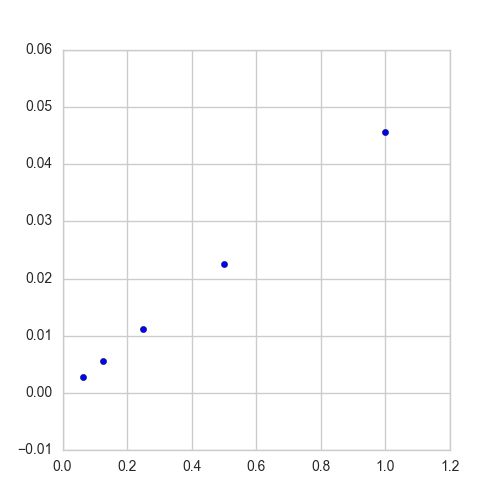
\includegraphics[scale=0.8]{manyErrors.png}
\end{center}

We see that the relationship between the maximum amplitude of the error on the interval $[0, 10\pi]$ and the value of $h$ is linear. They are directly proportional.

\section{Energy of the Approximation Over Time}

In a simple harmonic oscillator, the total energy is supposed to be conserved. We check the legitimacy of our approximation by looking at how the energy changes with time in our approximation. We plot the simple form of energy $(x^2+v^2) - 1$ against time, and also show the top portion of the error in $x(t)$ to compare the growth of the energy with the growth in amplitude of error. The reason we subtract the $1$ is to see the error and the energy on the same scale.

\begin{center}
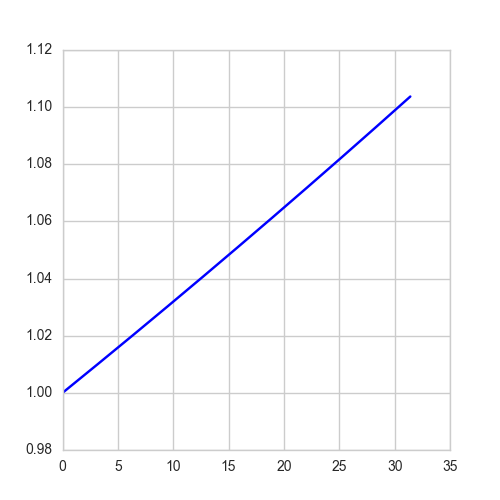
\includegraphics[scale=0.8]{energy.png}
\end{center}

\begin{center}
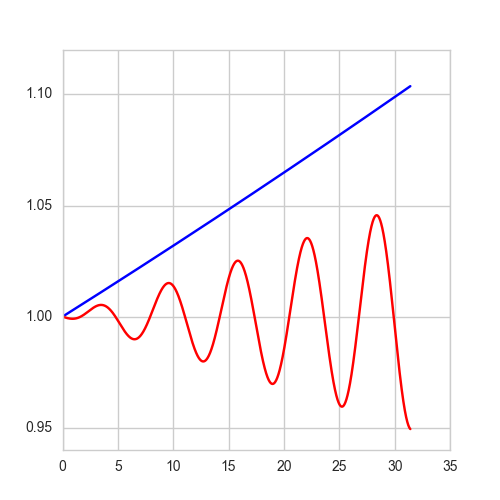
\includegraphics[scale=0.8]{energyWithErr.png}
\end{center}

We can see from the top figure that the energy does increase linearly with time. Looking at the bottom figure, the amplitude of the error also increases linearly. However, the energy increases at twice the rate of the error.

\section{The Implicit Euler Method}

The implicit Euler method is given by the matrix equation $$\begin{pmatrix} 1 & -h \\ h & 1 \end{pmatrix} \times \left( \begin{array}{c} x_{i+1}\\v_{i+1} \end{array} \right) = \left( \begin{array}{c} x_i\\v_i \end{array} \right)$$
We would like to solve this equation for expressions of $x_{i+1}$ and $v_{i+1}$ in terms of $x_i$ and $v_i$, respectively. We do this by inverting our two-by-two matrix. $${\begin{pmatrix} 1 & -h \\ h & 1 \end{pmatrix}}^{-1} = \frac{1}{1+h^2} \times \begin{pmatrix} 1 & h \\ -h & 1 \end{pmatrix}$$
Our matrix equation is then $$\left( \begin{array}{c} x_{i+1}\\v_{i+1} \end{array} \right) = \frac{1}{1+h^2} \times \begin{pmatrix} 1 & h \\ -h & 1 \end{pmatrix} \times \left( \begin{array}{c} x_i\\v_i \end{array} \right)$$
which reduces to $$\left( \begin{array}{c} x_{i+1}\\v_{i+1} \end{array} \right) = \frac{1}{1+h^2} \times \left( \begin{array}{c} x_i + hv_i\\-hx_i + x_i \end{array} \right)$$

\section{Comparison of the Implicit and Explicit Euler Methods}

Here we will look at graphics for the implicit Euler method calculated with $h=\frac{\pi}{1000}$. All of the figures are comparable to those shown for the explicit Euler method.

\begin{center}
\includegraphics[scale=0.8]{{impEulerOsc_x0_1.0_v0_0.0_h_0.003}.png}
\end{center}

Here we see that the explicit and implicit Euler methods each give sinusoids, but while the explicit Euler method shows an increasing amplitude, the implicit Euler method's amplitude decreases over time.

\begin{center}
\includegraphics[scale=0.8]{{impErrorOsc_x0_1.0_v0_0.0_h_0.003}.png}
\end{center}

When we analyze the error from the implicit Euler method, we see that the magnitude is identical to that of the explicit method. This means the implicit and explicit methods have the same rate of increase in error, and that one just is decreasing away from the actual solution and one is increasing away from it.

\begin{center}
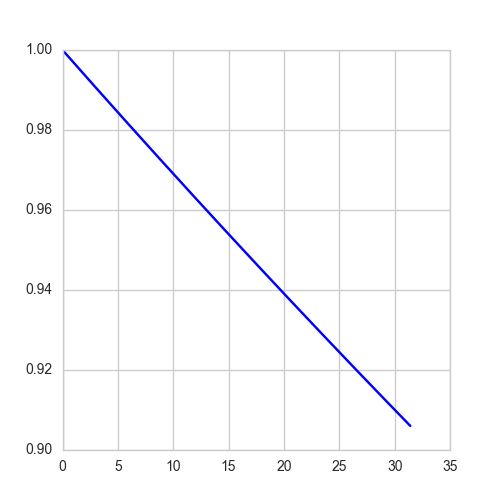
\includegraphics[scale=0.8]{impEnergy.png}
\end{center}

\begin{center}
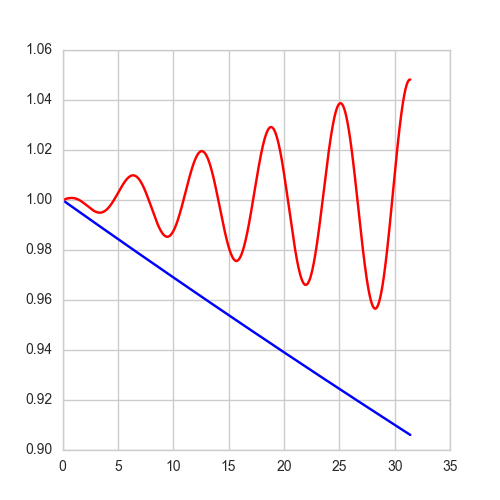
\includegraphics[scale=0.8]{impEnergyWithErr.png}
\end{center}

Now we can confirm the belief that the implicit and explicit solutions give mirror image approximations centered around the actual solution. We see above that the energy decreases linearly, and decreases twice as fast as the rate of change of the amplitude of the error, just as the explicit solution did. Thus the implicit and explicit solutions are equally effective, and neither is perfect.

\section{Symplectic Euler Method}

We will first look at the phase space plots of $x$ vs. $v$ for the explicit and implicit Euler methods. In these plots, we have set $h=\frac{\pi}{100}$.

\begin{center}
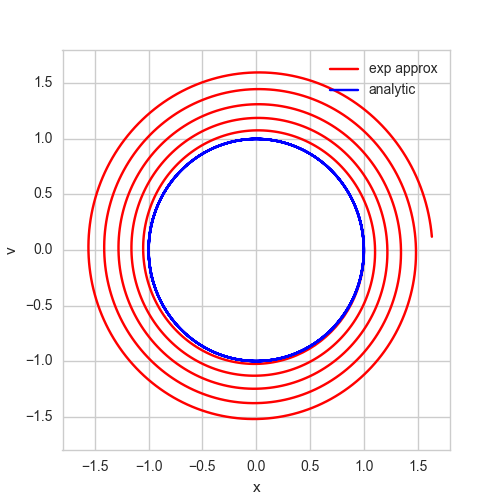
\includegraphics[scale=0.8]{expPhaseSpace.png}
\end{center}

\begin{center}
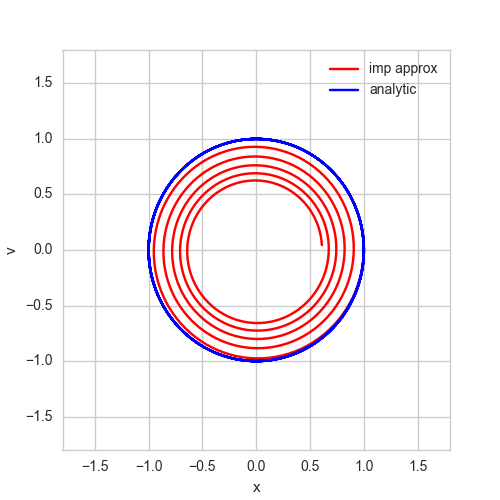
\includegraphics[scale=0.8]{impPhaseSpace.png}
\end{center}

We see that for the top figure, the plots spirals out, and for the bottom figure, the plot spirals in. The blue circle is the analytic solution, so we can see how the approximations spiral away from the analytic solution as $t$ increases.

\begin{center}
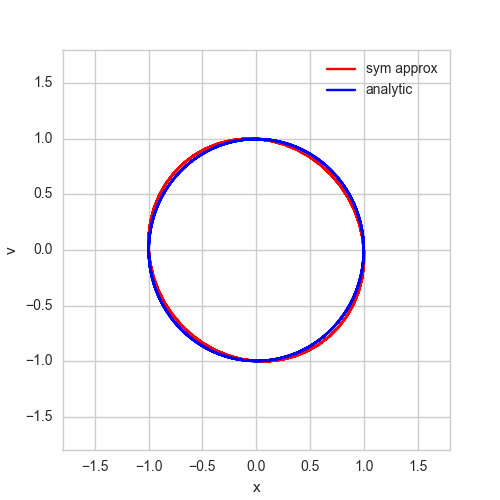
\includegraphics[scale=0.8]{symPhaseSpace.png}
\end{center}

\begin{center}
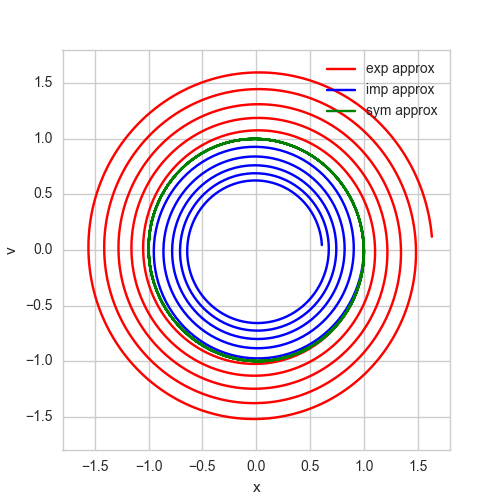
\includegraphics[scale=0.8]{allPhaseSpace.png}
\end{center}

Here we have added in the symplectic approximation, which is a middle ground between the implicit and explicit methods. We notice that in the top figure, where we have decreased $h$ to $\frac{\pi}{25}$, the symplectic approximation and the analytic solution are nearly indistinguishable in phase space. However, we can see that the symplectic approximation actually fluctuates slightly out and in relative to the analytic solution. In some areas, the two lines overlap perfectly, but elsewhere we can see both colors next to each other. This means the symplectic approximation does not perfectly approximate the analytic solution but instead oscillates around it. In the bottom figure, we remove the analytic solution and put all of the approximations together. Additionally, we return the $h$ for the symplectic approximation to $\frac{\pi}{100}$. Here we can see the difference between the approximations, and see how well the symplectic approximation preserves the analytic solution's phase space geometry compared to the other two.

\begin{center}
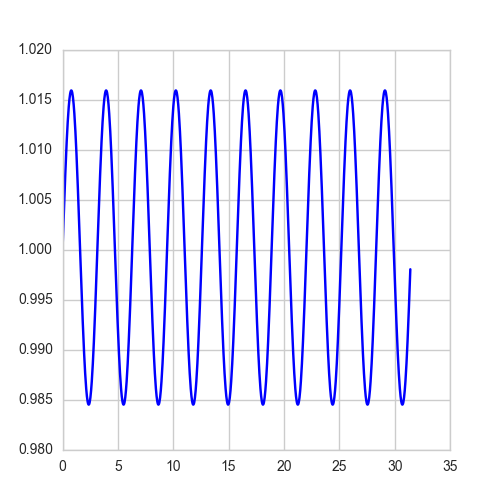
\includegraphics[scale=0.8]{symEnergy.png}
\end{center}

Now we can see that the symplectic approximation has fluctuating energy. The energy typically is centered around $x^2 + v^2 = 1$. The fluctuating energy explains the minute oscillations we see in the phase space figure for the symplectic approximation.

\end{document}